\documentclass[10pt]{article}

\usepackage{amsmath} \usepackage{amssymb} \usepackage{anysize}
\usepackage{amsthm} \usepackage{commath} \usepackage{float}
\usepackage{listings} \usepackage{graphicx}

\let\emptyset\varnothing

\marginsize{1in}{1in}{1in}{1in}
\title{\vspace{-2em}Site level interactions between intensive blood pressure management and
  adverse outcomes in SPRINT}
\author{Stats For Good}
\date{\today}

\begin{document} \maketitle

\begin{abstract}
  The SPRINT study defines a number of subgroup analyses to test for
  interactions between the treatment and other variables, for which they find no
  significance. With respect to the primary outcome, we find nonsignificance
  for most relevant baseline variables. Beyond this, we argue that interactions
  between treatment site and the intensive treatment are interesting to
  consider, and use statistical analysis to demonstrate there are plausible
  interactions that deserve further investigation. 
\end{abstract}

\section{Covariate interactions}
\subsection{Methods}
We considered pairwise interactions of race, gender, BMI, smoking status, and
medications (aspirin and statins) with the intensive versus standard
treatment. We first considered the incidence of any condition in the
primary endpoint (TODO add exact vars included) within 5 years as our outcome,
and considered a Cox proportional hazards regression model. We also considered
interactions between the baseline covariates listed above and the treatment
against severe adverse outcomes.

Further, we investigated the possibility that subgroups defined via specific
thresholds of baseline covariates may have stronger interactions with the
treatment variable. To this end, we fit an honest decision tree (TODO: add
citation to Athey and Imbens) with the binary outcome of incidence of primary
CVD within 5 years.

\subsection{Results}
No interactions were significant for primary outcomes (P > 0.1) or severe
adverse events (P > 0.1). In the fitted causal tree, BMI was the only variable
considered in the top two layers of the tree, so we considered the average
treatment effect of the intensive treatment in each decile of BMI, included in
Figure (TODO: make into figure), in which no clear trend is apparent. 

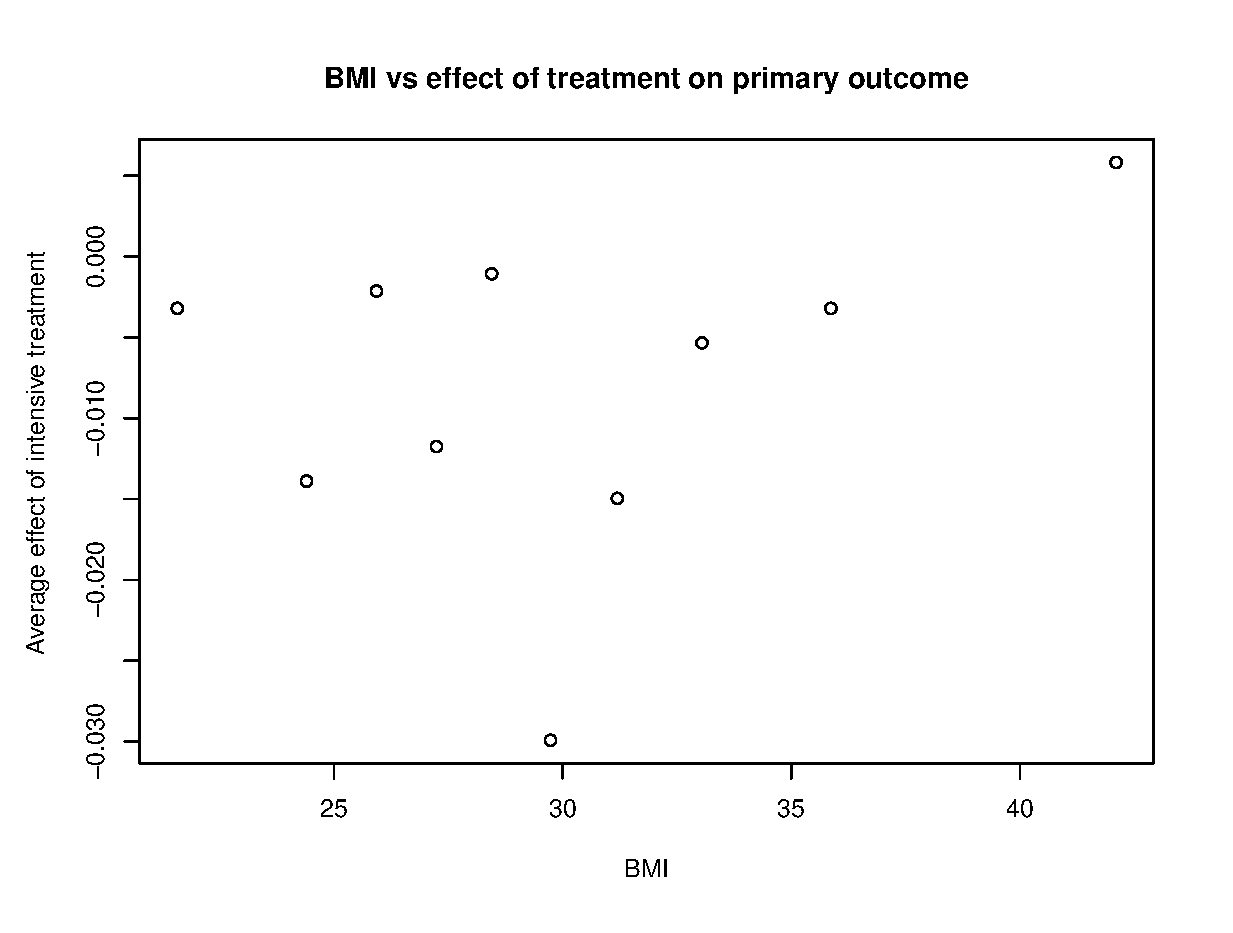
\includegraphics[width=3.5in]{ate_bmi_interaction.eps}

\section{Site specific outcomes}
\subsection{Methods}
TODO: include explanation of how networks were identified.
Among the networks identified, we tested for interactions between the provider
network as a categorical factor, and the intensive treatment against adverse
events as the outcome. All individuals who were a part of the study but not one
of the five identifiable networks were included as a baseline factor. We fit a
multivariate proportional hazards Cox model to these data, and looked for
significance at the $P = 0.1$ and $P=0.05$ levels.

\subsection{Results}
TODO: convert to table
The following number of individuals were found to be in each of the networks
identified. NA is used as a placeholder for all sites that were not identified.

\begin{center}
\begin{tabular}{ |c|l|r| } 
 \hline
 &      \textbf{NET}&   \textbf{n} \\
 \hline
1&       NA&5285 \\
 \hline
2&     OHIO& 844 \\
 \hline
3&SOUTHEAST& 773 \\
 \hline
4      &UAB& 489 \\
 \hline
5      & VA&1970 \\
 \hline
\end{tabular}
\end{center}


Among these sites, the interaction between the intensive treatment and the
Southeast network was found to be significant at $P = 0.068$, with a negative
interaction. That is, individuals in the Southeast network were less likely to
have a severe adverse event mediated by the intensive versus standard treatment
than the average individual in the study.

\subsection{Conclusions}
The significance for the network level interactions found was inconclusive,
however it warrants further investigation. As the study was not powered to
consider these geographic interactions with respect to adverse events, the data
derived from the SPRINT study provide an exploratory look at considering these
interactions. The first step would be analysis with the un-anonymized site
information, followed by a RCT powered to understand how demographic and
geographic factors mediate the adverse effects of intensive blood pressure
management.

\end{document}